% MU 夜间/日内策略 — 总评估报告 (XeLaTeX)
% latexmk -xelatex final_report.tex
\documentclass[11pt,a4paper,fontset=none]{ctexart}
\setCJKmainfont{Noto Serif CJK SC}
\setCJKsansfont{Noto Sans CJK SC}
\setCJKmonofont{Noto Sans Mono CJK SC}

\usepackage[margin=2.3cm]{geometry}
\usepackage{graphicx,booktabs,float,amsmath,longtable}
\usepackage[table]{xcolor}
\usepackage{caption}
\captionsetup{font=small,labelfont=bf}
\usepackage[colorlinks=true,linkcolor=blue!55!black,urlcolor=blue!55!black,citecolor=blue!55!black]{hyperref}
\usepackage{xurl}

\definecolor{good}{RGB}{26,127,55}
\definecolor{bad}{RGB}{207,34,46}
\definecolor{hl}{RGB}{250,240,200}
\newcommand{\pos}[1]{\textcolor{good}{#1}}
\newcommand{\negv}[1]{\textcolor{bad}{#1}}
\graphicspath{{fig/}}

\title{\bfseries 夜间 vs 日内收益策略：总评估报告\\
\large Overnight--Intraday Return Gap 的现象验证、市场状态分解、策略评估与实操框架\\[2pt]
\normalsize 核心样本：美光科技 (MU) ｜ 横截面：22 只标的}
\author{TradeMind}
\date{2026 年 6 月 8 日}

\begin{document}
\maketitle

\begin{center}
\colorbox{hl}{\parbox{0.95\textwidth}{\small
\textbf{执行摘要（一页结论）}\\[3pt]
\textbf{1. 现象真实}：夜间腿（收盘→次日开盘）在 MU 上 42 年 $t=9.15$，全部长期涨幅来自隔夜；日内腿累计为负。横截面 22 票中 15 票显著，集中于高波动成长/半导体股。\\[2pt]
\textbf{2. 但不是提款机}：盈亏平衡成本约 7.8 bps/单边。零成本 280 万倍是复利神话，5 bps 即跑输买入持有，10 bps 归零。所谓"1.38 亿\%"是网红误读，非论文结论。\\[2pt]
\textbf{3. 本质是牛市现象}：牛市 18/22 票显著；熊市仅 1 票（AMD）幸存、9 票转负，日内腿反而反超——"拔河"方向在熊市掉头。\\[2pt]
\textbf{4. 对下跌的保护是有条件的}：盘中阴跌型熊市大幅减亏；隔夜跳空型熊市（COVID、2022）不减亏反略扩大，且隔夜持仓无法止损。\\[2pt]
\textbf{5. 最有价值的产物是趋势过滤}：只在个股位于自身 200 日线上方持隔夜，把最大回撤从 $-69\%$ 砍到 $-34\%$、波动从 28\% 降到 19\%、Sharpe 从 1.05 升到 1.22（含 2 bps 成本）。\\[2pt]
\textbf{6. "多夜空日"对冲不可行}：该价差为市场中性、毛收益更高，但换手翻倍、做空一个统计不显著的腿、熊市归零（$t=-0.04$）、5 bps 即转负——散户净亏，且它\emph{不}对冲方向性多头。
}}
\end{center}

\tableofcontents
\newpage

%==========================================================
\section{背景与起因}
\subsection{起因：一条把现象讲成"阴谋"的病毒式推文}
本研究的直接触发，是 2026 年 6 月 6 日 X（Twitter）用户 \textbf{柴郡｜Crypto+AI Plus（@0xCheshire）} 发布的一条引发热议的帖子（\href{https://x.com/0xCheshire/status/2063111971013263404}{链接}）。该帖的核心要点为：

\begin{itemize}\itemsep0pt
  \item 称美光（MU）"\textbf{收盘买入、次日开盘卖出}"几十年累计收益 \textbf{+138{,}330{,}342\%}；
  \item 而反向的"开盘买入、收盘卖出"累计 \textbf{$-$99.92\%}；
  \item 将此现象渲染为"\textbf{波及所有市场、包括 A 股的某种操纵/阴谋}"。
\end{itemize}

值得注意的是，X 的\textbf{社区注释（Community Notes）已对该帖纠偏}：指出这其实是学术界早已记录的"隔夜收益之谜（overnight returns puzzle）"，其回测\emph{未计入交易成本}，且 A 股在 T+1 制度下隔夜收益实际为\emph{负}——与"所有市场一样"的说法相悖。本报告的立场与该社区注释一致：\textbf{现象真实、机制有学术解释，但"阴谋"与"无脑套利"两种叙事都是误读}。

\subsection{白话翻译：论文到底在说什么}
把学术语言翻译成人话——它\emph{不是}在说"美光有黑幕"或"有人白天砸盘晚上拉盘"，而是在说一件结构性的事实：

\begin{quote}
同一只股票，一天里的"\textbf{夜间收益}"（收盘$\to$次日开盘）和"\textbf{日内收益}"（开盘$\to$收盘）不是同一种东西。有些股票的长期上涨几乎全部发生在"收盘$\to$开盘"这段，而"开盘$\to$收盘"这段长期很弱、甚至为负。
\end{quote}

于是"收盘买、开盘卖"与"开盘买、收盘卖"两条路径的长期复利会差到极其夸张。那个吓人的 1.38 亿\% \textbf{不是单日神迹，而是"每天一点点正期望 $\times$ 几十年复利 $\times$ 假设理想成交价"的放大结果}——这正是本报告 §3、§5 要量化的东西。

\subsection{为什么会这样：四类学术解释}
\begin{enumerate}\itemsep2pt
  \item \textbf{交易人群不同（拔河 / tug of war）}：散户更倾向开盘附近下单、机构更倾向收盘附近执行，两类资金方向不同，造成价格在日内与夜间被反向"拉扯"。这是 Lou--Polk--Skouras 的核心机制，也与本报告 $\rho=0.51$（波动/散户关注越高、效应越强）的发现吻合。
  \item \textbf{时段流动性与价格压力不同}：开盘释放隔夜累积订单、收盘有指数基准与结算的集中交易，两个时点的冲击成本结构不同。
  \item \textbf{夜间信息一次性反映}：财报、指引、宏观数据、海外市场、地缘新闻多在盘后出现，开盘一次性定价——"夜间涨"部分是\emph{对承担隔夜风险的补偿}。
  \item \textbf{A 股的制度差异（方向性判断，本报告未回测）}：T+1、散户占比高、涨跌停、市场不连续等会改变日夜行为；但如社区注释所言，A 股隔夜收益常为负，机制与美股\emph{不同}，"所有市场一样"过于粗暴。
\end{enumerate}

\subsection{论文的真实主张（学术精确版）}
核心文献 Lou--Polk--Skouras《A Tug of War》(JFE 2019) 的结论是一个\textbf{统计分解命题}：一只股票的收益可拆为\emph{夜间}与\emph{日内}两个持续、可预测、常方向相反的成分；长期平均看夜间成分期望收益显著为正、日内接近零或为负。它说的是\textbf{期望收益}（长期平均）、是\textbf{成分分解}、且明确是一个\textbf{异象}（未扣成本）。

\subsection{常见误读（错的不是论文，是二次转述）}
\begin{table}[H]\centering\small
\begin{tabular}{p{6cm}p{8.5cm}}
\toprule
病毒式说法 & 为什么错 \\
\midrule
"收盘买开盘卖能赚 1.38 亿\%" & 零成本 + 42 年复利的算术产物；扣 5 bps 只剩 71 倍，扣 10 bps 归零 \\
"夜间策略稳赚 / 躺赢" & 论文从未声称在任何窗口都赢买入持有 \\
"波及所有市场的阴谋" & 学界早有解释（拔河/流动性/信息/风险补偿）；A 股 T+1 下隔夜反为负 \\
"这是无脑套利" & 论文白纸黑字写明是 anomaly，非 free lunch \\
\bottomrule
\end{tabular}
\caption{本报告全程证实论文、否定误读。最后两行直接对应推文与其社区注释。}
\end{table}

\subsection{原始来源与文献链接}
\textbf{起因（推文）}：
\begin{itemize}\itemsep0pt
  \item 柴郡 @0xCheshire（2026-06-06）：\url{https://x.com/0xCheshire/status/2063111971013263404}
\end{itemize}
\textbf{论文原文}：
\begin{itemize}\itemsep0pt
  \item Lou, Polk, Skouras, \textit{A Tug of War: Overnight versus Intraday Expected Returns}, JFE 2019：\\
        出版页 \url{https://www.sciencedirect.com/science/article/abs/pii/S0304405X19300650}；\\
        作者 PDF（LSE）\url{https://personal.lse.ac.uk/polk/research/TugOfWar.pdf}
  \item \textit{Does Overnight News Explain Overnight Returns?}（2025，分析 240 万篇新闻）：\url{https://arxiv.org/abs/2507.04481}
  \item \textit{Overnight-Intraday Return Gap and the Retail Ebb and Flow}（SSRN）：\url{https://papers.ssrn.com/sol3/papers.cfm?abstract_id=4752520}
  \item \textit{Night Moves: Is the Overnight Drift the Grandmother of All Market Anomalies?}（JOIM）：\url{https://www.joim.com/wp-content/uploads/emember/downloads/P0753.pdf}
  \item \textit{The Asymmetric Overnight Return Anomaly in the Chinese Stock Market}（MDPI，A 股）：\url{https://www.mdpi.com/1911-8074/15/11/534}
\end{itemize}
\textbf{权威解读与反方质疑（与本报告结论一致）}：
\begin{itemize}\itemsep0pt
  \item Elm Wealth（Victor Haghani），\textit{Night Moves}：\url{https://elmwealth.com/night-moves-overnight-drift/}
  \item AlphaArchitect，\textit{Trading Costs Wipe Out the Overnight Return Anomaly}（标题即结论，印证本报告 §5）：\url{https://alphaarchitect.com/trading-costs-wipe-out-the-overnight-return-anomaly/}
  \item Nasdaq，\textit{Like Night and Day}：\url{https://www.nasdaq.com/articles/night-and-day}
\end{itemize}

%==========================================================
\section{方法与数据}
\subsection{收益拆分}
\begin{align}
r^{\text{overnight}}_t = \frac{\text{Open}_t}{\text{Close}_{t-1}} - 1, \qquad
r^{\text{intraday}}_t = \frac{\text{Close}_t}{\text{Open}_t} - 1, \qquad
r^{\text{cc}}_t = (1+r^{\text{on}}_t)(1+r^{\text{in}}_t)-1
\end{align}
关键恒等式：\textbf{买入持有 = 夜间腿 $\circ$ 日内腿}（两段复利相乘）。这是后文一切对比的基础——买入持有同时吃两段，夜间策略只吃一段。

\subsection{数据与成本}
\begin{itemize}\itemsep0pt
  \item 数据源：Yahoo Finance 日线 OHLC，前复权（分红、拆股已并入）；
  \item MU：1984-06-04 至 2026-06-05，共 10{,}584 个交易日；横截面 22 票统一自 2000 年起；
  \item 成本：每笔成交单边 $c\in\{0,2,5,10\}$ bps；单腿策略每天 2 笔，价差策略每天 4 笔；
  \item 状态判定全部用 $t-1$ 收盘可得信息（SPY/个股 MA200、前日涨跌），无前视偏差。
\end{itemize}

%==========================================================
\section{MU 核心绩效}
\begin{figure}[H]\centering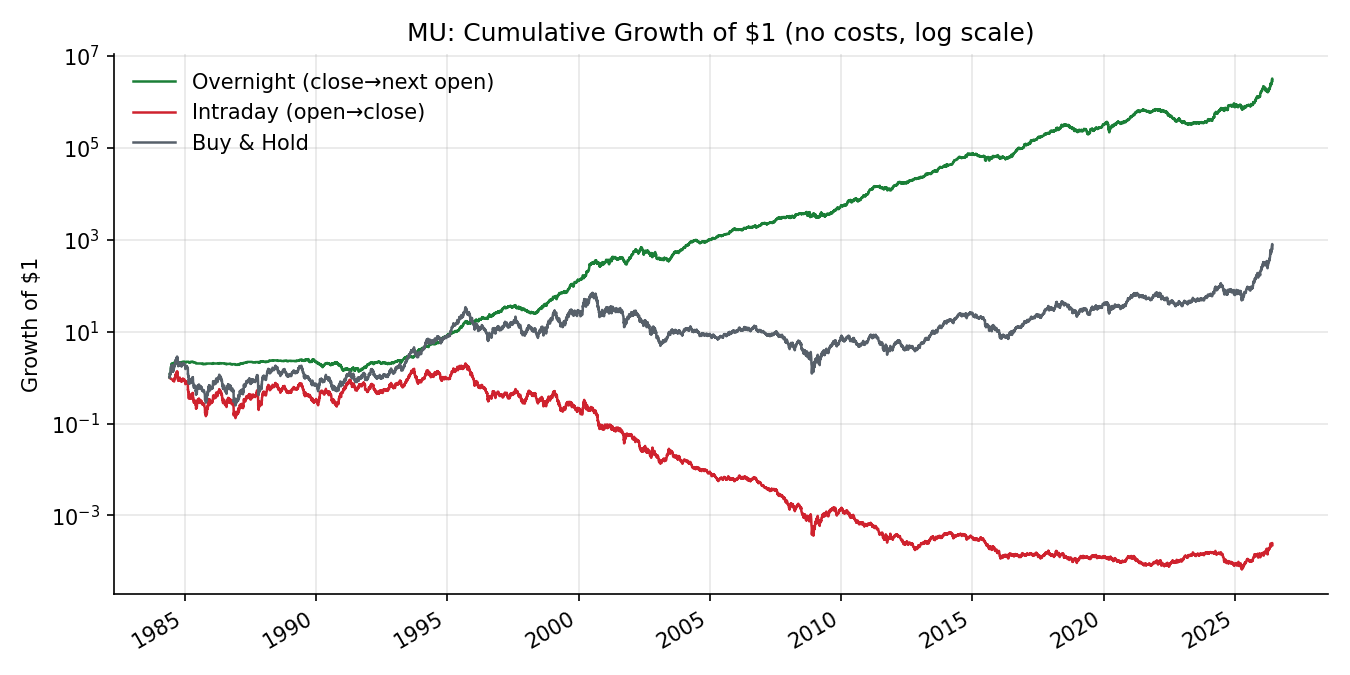
\includegraphics[width=\textwidth]{fig1_equity.png}
\caption{三条腿累计净值（零成本，对数轴）。夜间腿 42 年 $2.8\times10^6$ 倍即天文数字来源；日内腿归零；买入持有 640 倍恰为两者之积。}\end{figure}

\begin{table}[H]\centering\small
\begin{tabular}{lrrrrrrrr}
\toprule
策略 & 成本 & 日均(bps) & $t$ & Sharpe & Sortino & CAGR & 累计 & MaxDD \\
\midrule
夜间 & 0 & \pos{+15.6} & \pos{9.15} & 1.41 & 1.78 & \pos{+42.4\%} & 280万$\times$ & $-$54\% \\
夜间 & 2 & \pos{+11.6} & \pos{6.80} & 1.05 & 1.39 & \pos{+28.8\%} & 4.07万$\times$ & $-$69\% \\
夜间 & 5 & \pos{+5.6} & \pos{3.27} & 0.50 & 0.67 & \pos{+10.7\%} & 71$\times$ & $-$89\% \\
夜间 & 10 & \negv{$-$4.5} & \negv{$-$2.62} & $-$0.40 & $-$0.55 & \negv{$-$14.0\%} & 归零 & $-$100\% \\
日内 & 0 & \negv{$-$2.4} & $-$0.73 & $-$0.11 & $-$0.17 & \negv{$-$18.1\%} & 归零 & $-$100\% \\
买入持有 & --- & +13.4 & 3.61 & 0.56 & 0.84 & +16.6\% & 640$\times$ & $-$98\% \\
\bottomrule
\end{tabular}
\caption{MU 全样本绩效。夜间腿偏度 $+0.11$、峰度 $11.2$，厚尾显著。}\end{table}

\begin{figure}[H]\centering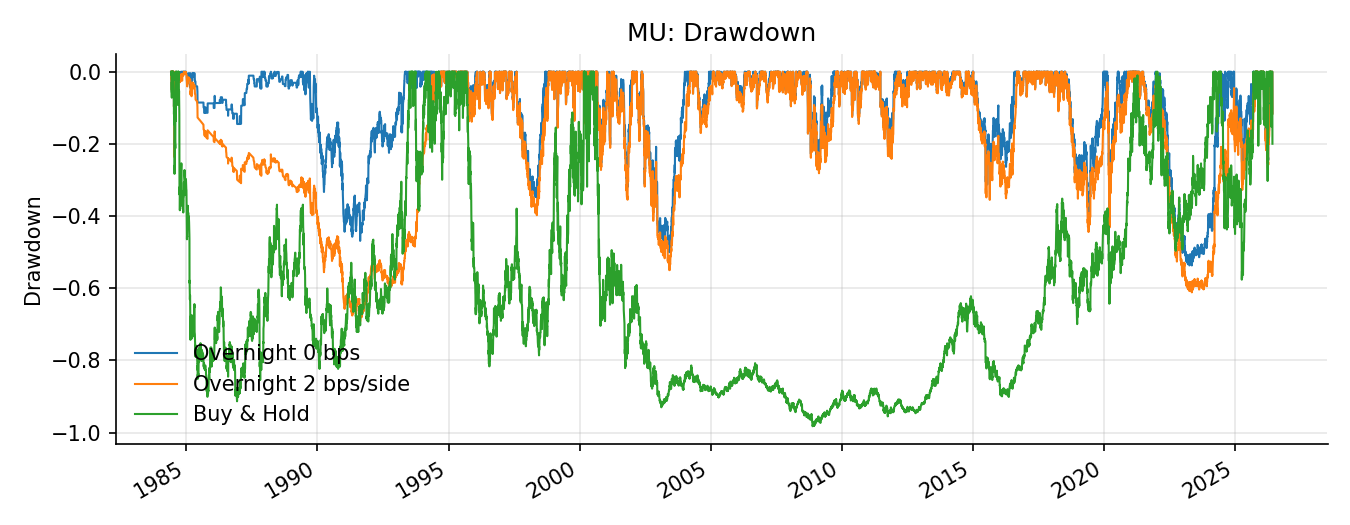
\includegraphics[width=\textwidth]{fig2_drawdown.png}
\caption{回撤曲线。夜间腿并非低风险：零成本 $-54\%$、2 bps 达 $-69\%$，只是浅于买入持有的 $-98\%$。}\end{figure}

\begin{figure}[H]\centering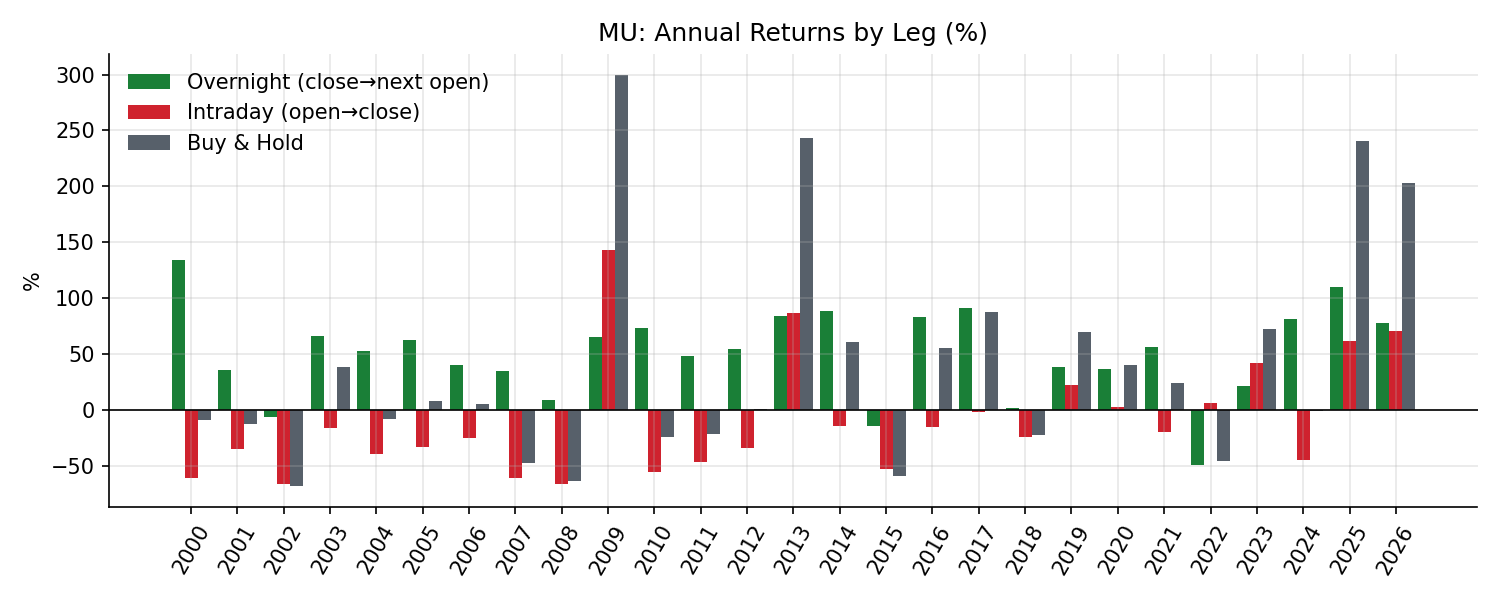
\includegraphics[width=\textwidth]{fig3_yearly.png}
\caption{分年度收益（2000 起）。2022 年夜间腿 $-49\%$、2023 年日内反超——效应有大小年。2026 为不完整年度。}\end{figure}

\begin{figure}[H]\centering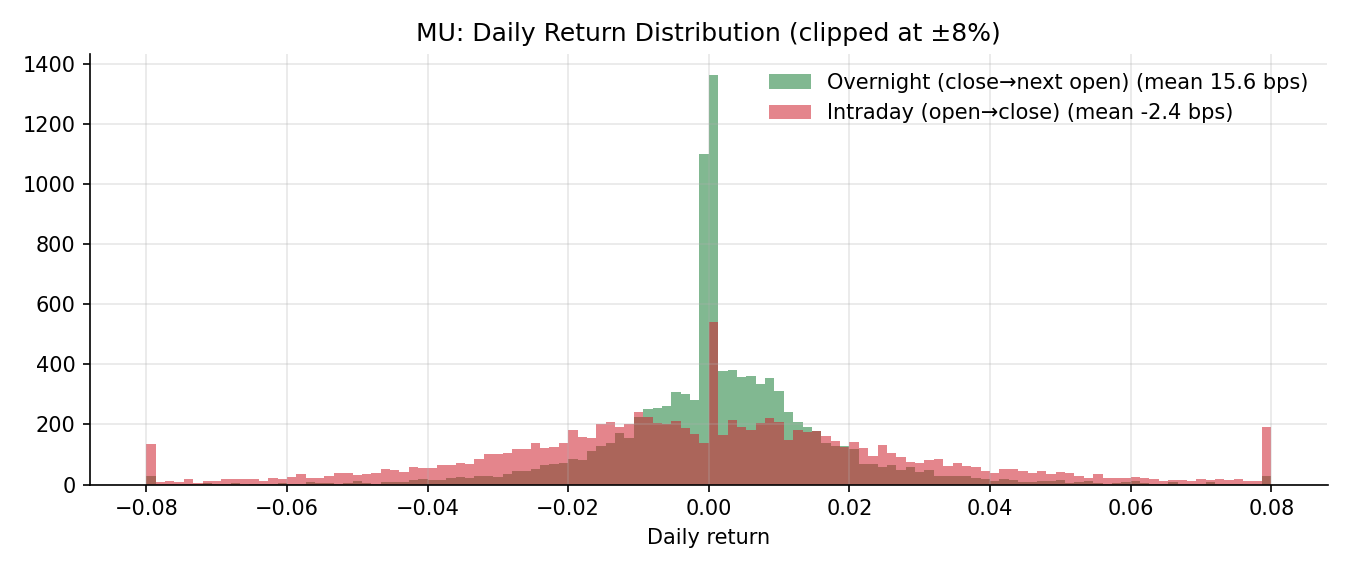
\includegraphics[width=\textwidth]{fig6_dist.png}
\caption{日收益分布。两腿形状几乎相同，差异仅在均值的细微平移（$+15.6$ vs $-2.4$ bps）——肉眼不可见的日度优势靠复利放大。}\end{figure}

%==========================================================
\section{稳健性}
\begin{figure}[H]\centering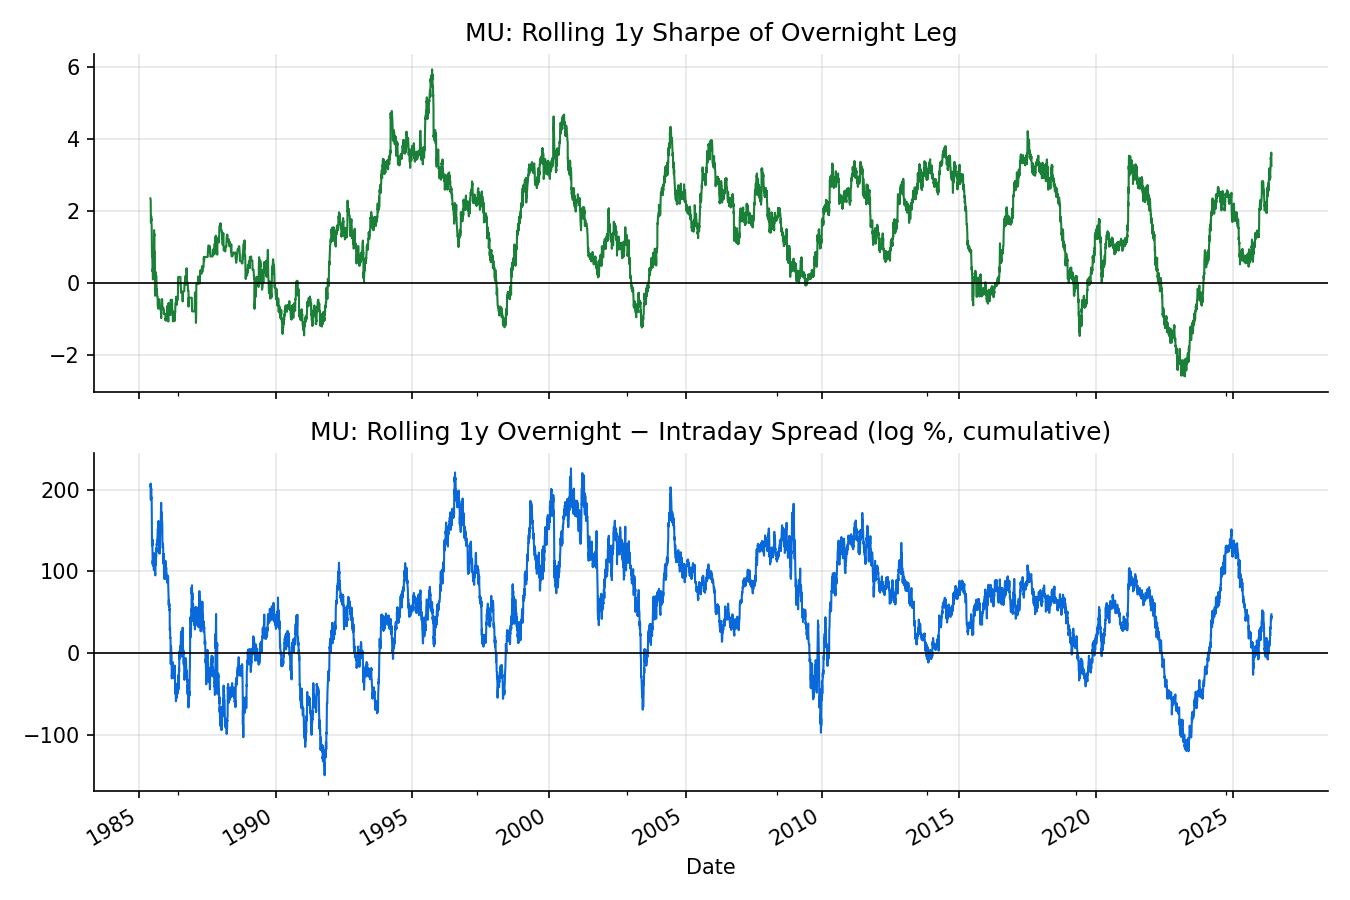
\includegraphics[width=\textwidth]{fig4_rolling.png}
\caption{上：夜间腿滚动 1 年 Sharpe，18.6\% 的时间为负；下：滚动 1 年"夜间$-$日内"价差，长期为正但 2022 深度转负。}\end{figure}

\begin{figure}[H]\centering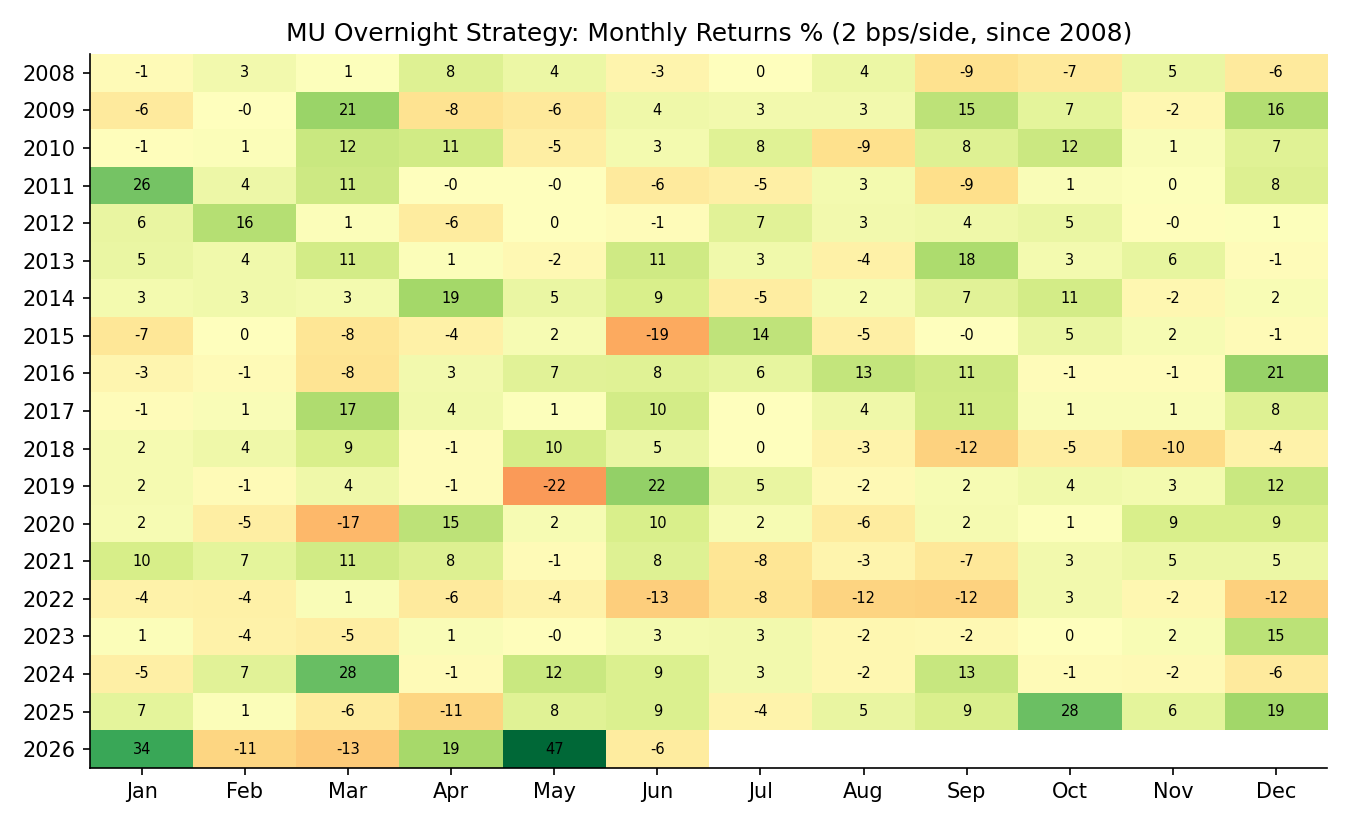
\includegraphics[width=0.92\textwidth]{fig5_heatmap.png}
\caption{夜间策略（2 bps）月度热力图。红色连片于 2008/2015/2018/2022——系统性风险期同样亏损。}\end{figure}

\subsection{成本：策略的生死线}
\begin{figure}[H]\centering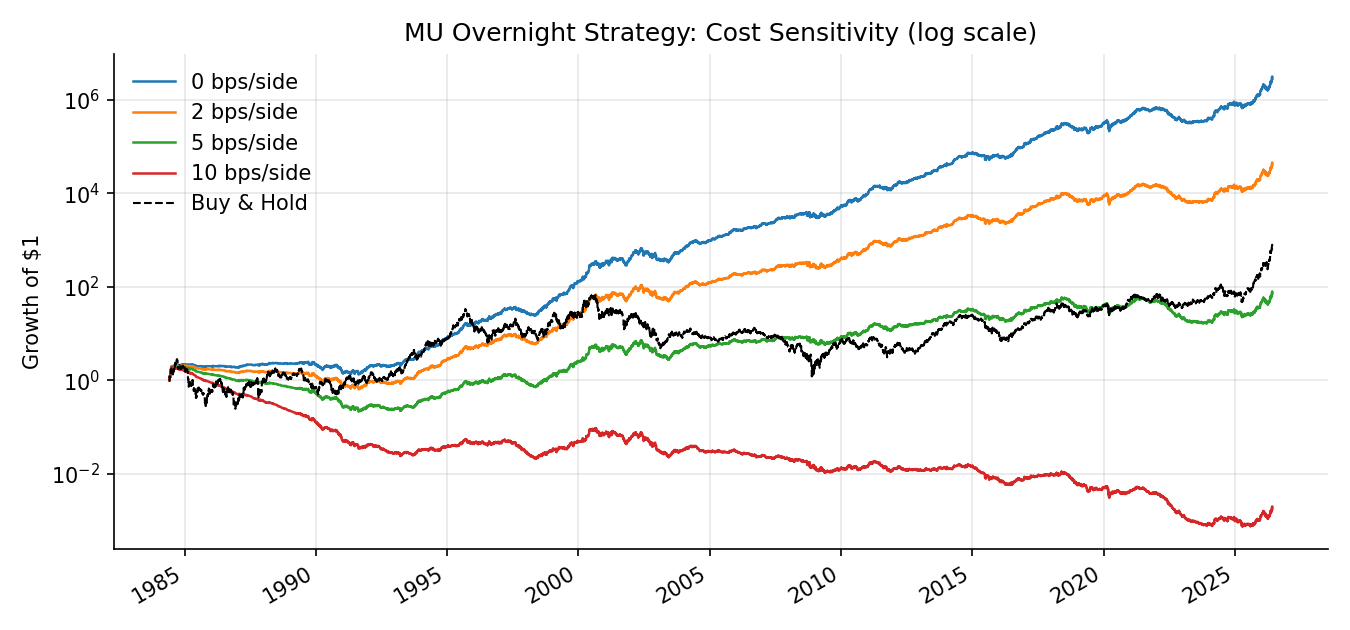
\includegraphics[width=\textwidth]{fig7_cost.png}
\caption{成本敏感性。盈亏平衡 $\approx 7.8$ bps/单边：2 bps 跑赢买入持有，5 bps 落后，10 bps 归零。}\end{figure}

\subsection{需要持有多久才能盈利}
\begin{figure}[H]\centering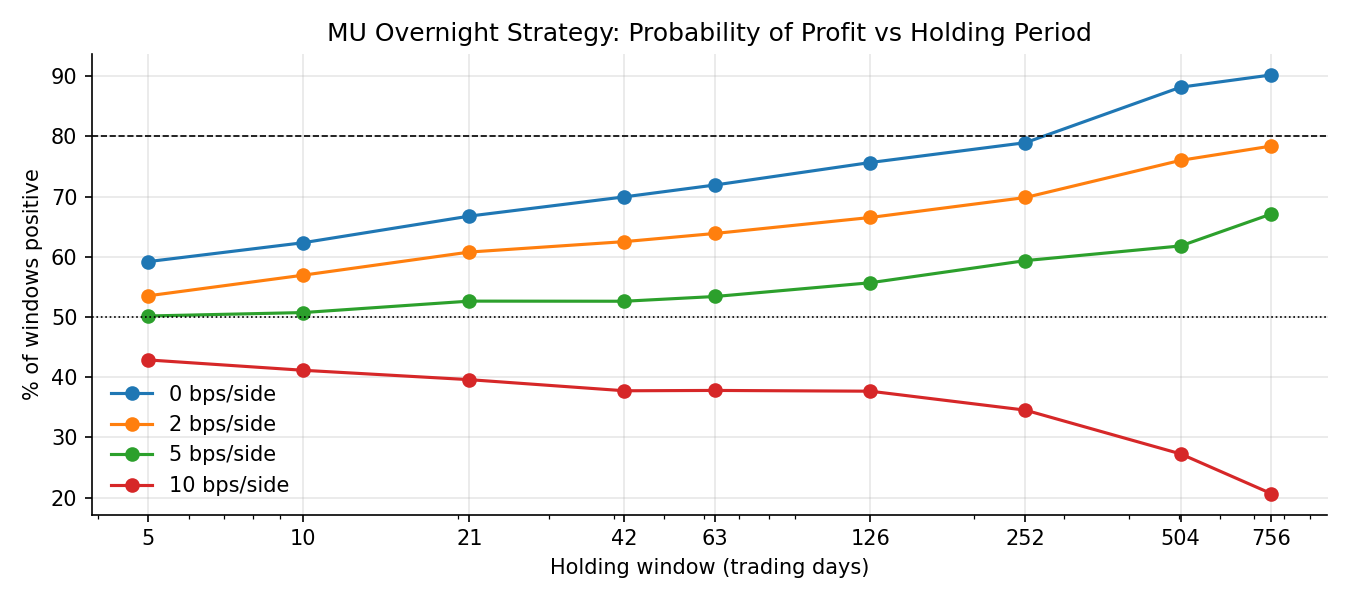
\includegraphics[width=\textwidth]{fig8_days_to_profit.png}
\caption{滚动 $N$ 日正收益概率。零成本约 2 年（504 日）达 88\%；2 bps 下 3 年仅 78\%；5 bps 短期近抛硬币。无"保证盈利天数"。}\end{figure}

%==========================================================
\section{横截面：在什么股票上生效}
\begin{figure}[H]\centering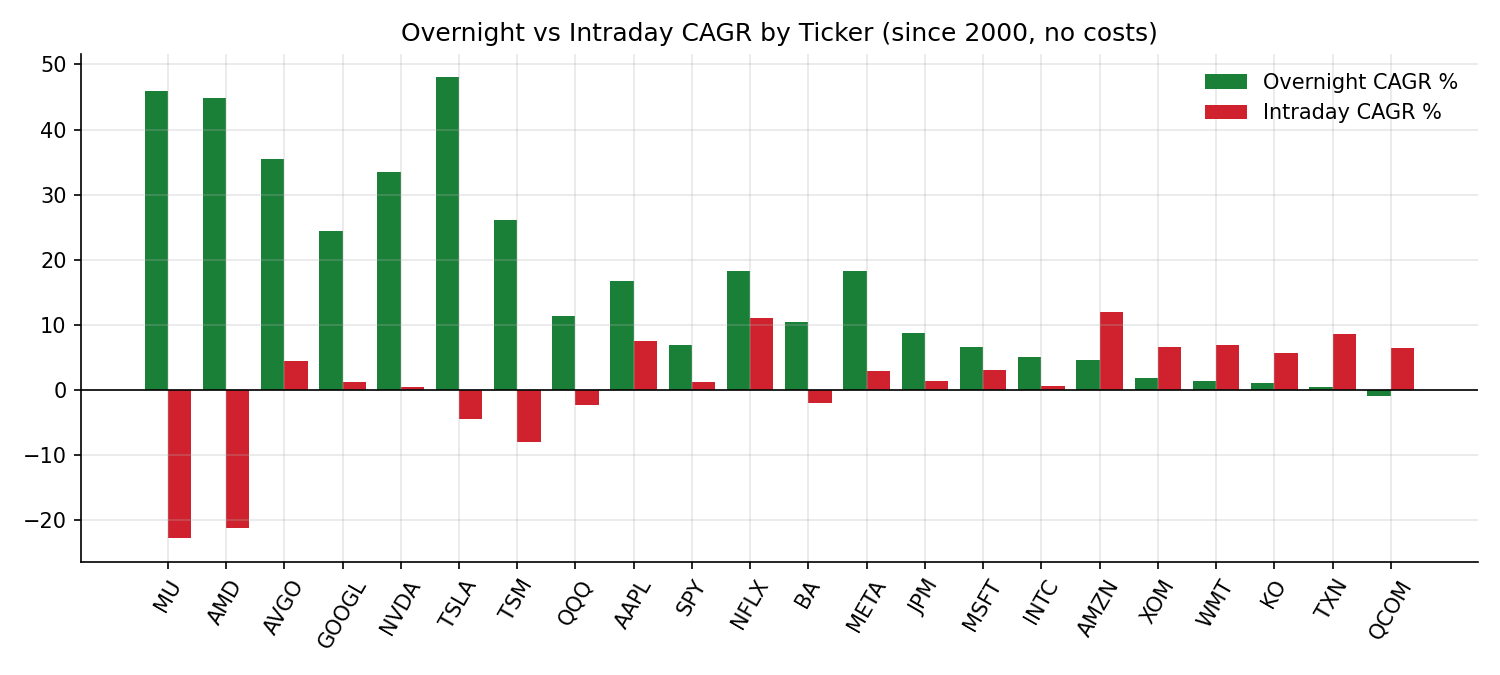
\includegraphics[width=\textwidth]{fig9_universe.png}
\caption{22 票夜间 vs 日内 CAGR（2000 起，零成本）。左侧绿柱领先者全为高波动半导体/成长股；右端价值股红柱反超。}\end{figure}

\begin{figure}[H]\centering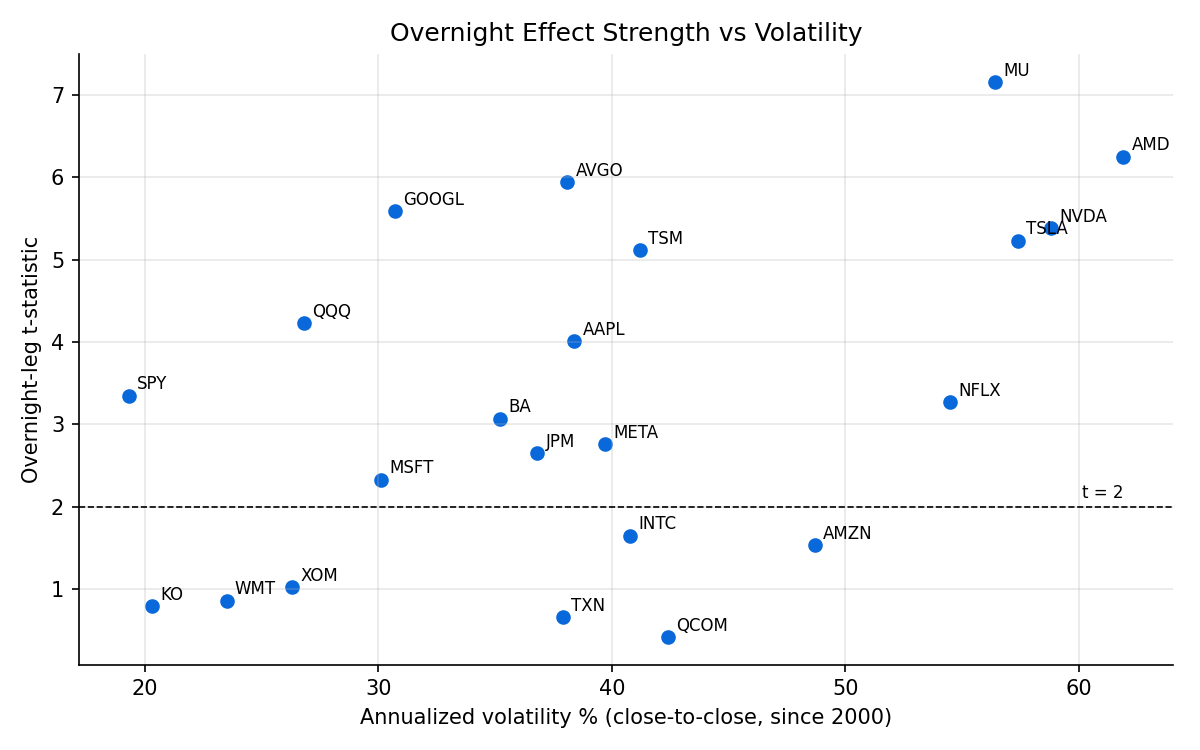
\includegraphics[width=0.78\textwidth]{fig10_scatter.png}
\caption{效应强度与波动率正相关（$\rho=0.51$）——波动越高、散户关注越高，夜间效应越强，符合"拔河"机制。}\end{figure}

\begin{table}[H]\centering\small
\begin{tabular}{lp{7cm}c}
\toprule
分组 & 标的（夜间 $t$） & 判定 \\
\midrule
强生效 ($t>5$) & MU(7.2) AMD(6.3) AVGO(5.9) GOOGL(5.6) NVDA(5.4) TSLA(5.2) TSM(5.1) & \pos{显著} \\
弱生效 ($2<t<5$) & QQQ AAPL SPY NFLX BA META JPM MSFT & \pos{显著} \\
不生效 ($t<2$) & INTC AMZN XOM WMT KO TXN QCOM & \negv{日内反超} \\
\bottomrule
\end{tabular}
\caption{横截面分组：22 票中 15 票显著。}\end{table}

%==========================================================
\section{市场状态：牛熊与涨跌}
\begin{table}[H]\centering\small
\begin{tabular}{lrrrr}
\toprule
状态 & 夜间均值(bps,22票) & 显著票数 & 日内均值(bps) & 谁占优 \\
\midrule
牛市 (SPY$>$MA200) & \pos{+8.6} & \pos{18/22} & +0.7 & 夜间压倒 \\
熊市 (SPY$<$MA200) & +2.1 & \negv{1/22} & \pos{+7.6} & \negv{日内反超} \\
\bottomrule
\end{tabular}
\caption{牛熊是夜间效应的第一决定因素。熊市唯一显著的是 AMD；NVDA/TSM/AAPL/AMZN/NFLX 等 9 票转负。}\end{table}

\begin{figure}[H]\centering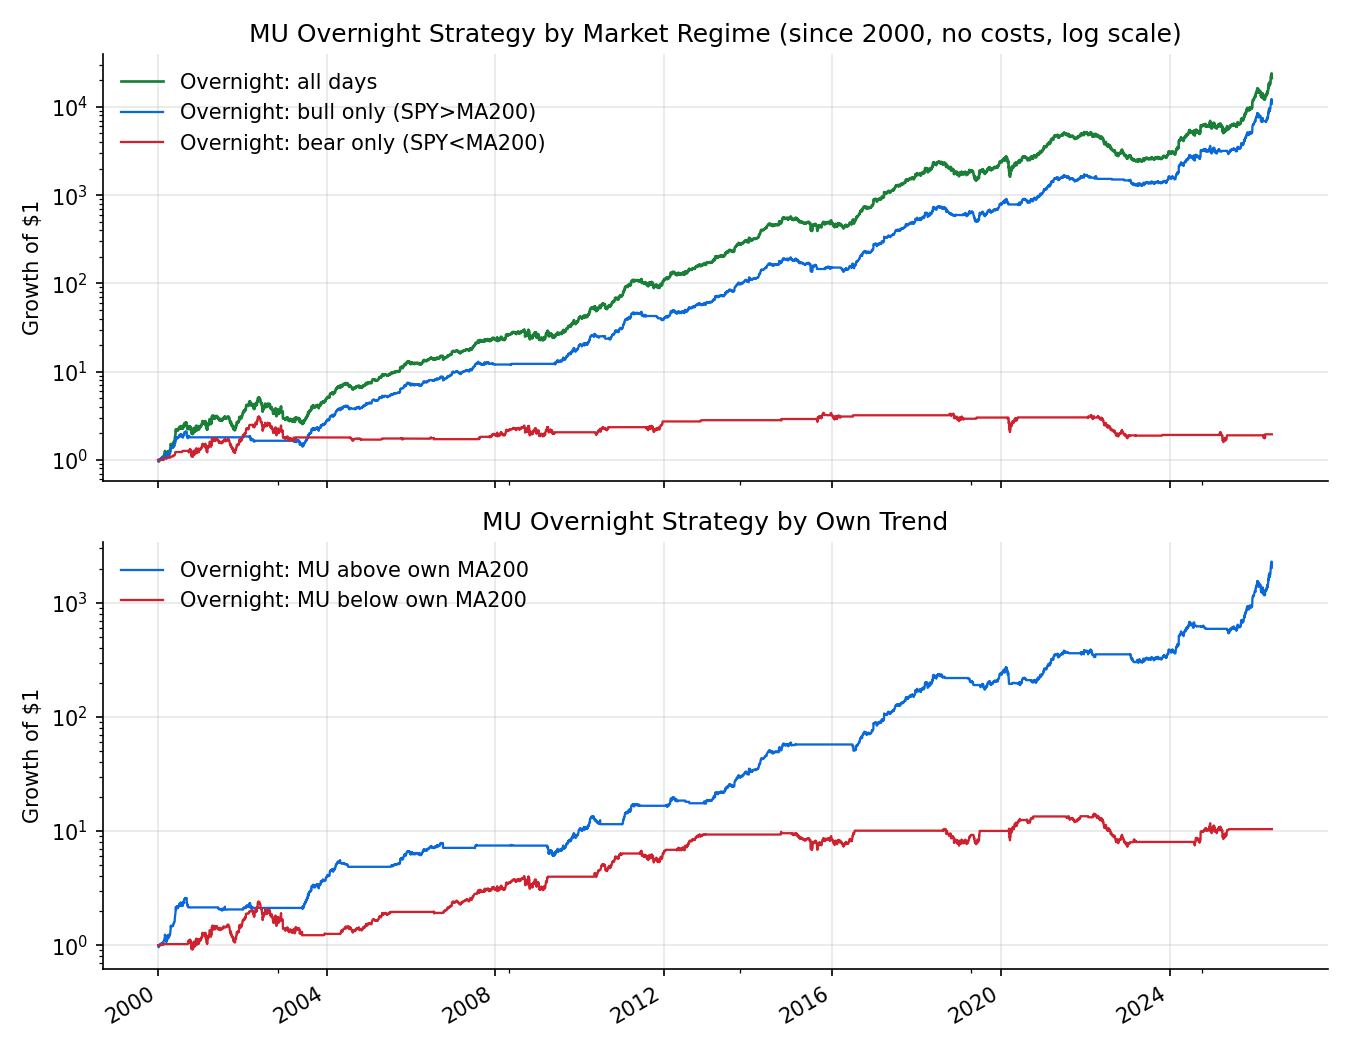
\includegraphics[width=0.92\textwidth]{fig11_regime_equity.png}
\caption{MU 夜间策略按状态拆分。上：牛市贡献绝大部分收益，熊市段近乎走平；下：自身趋势过滤区分度更高。}\end{figure}

\begin{figure}[H]\centering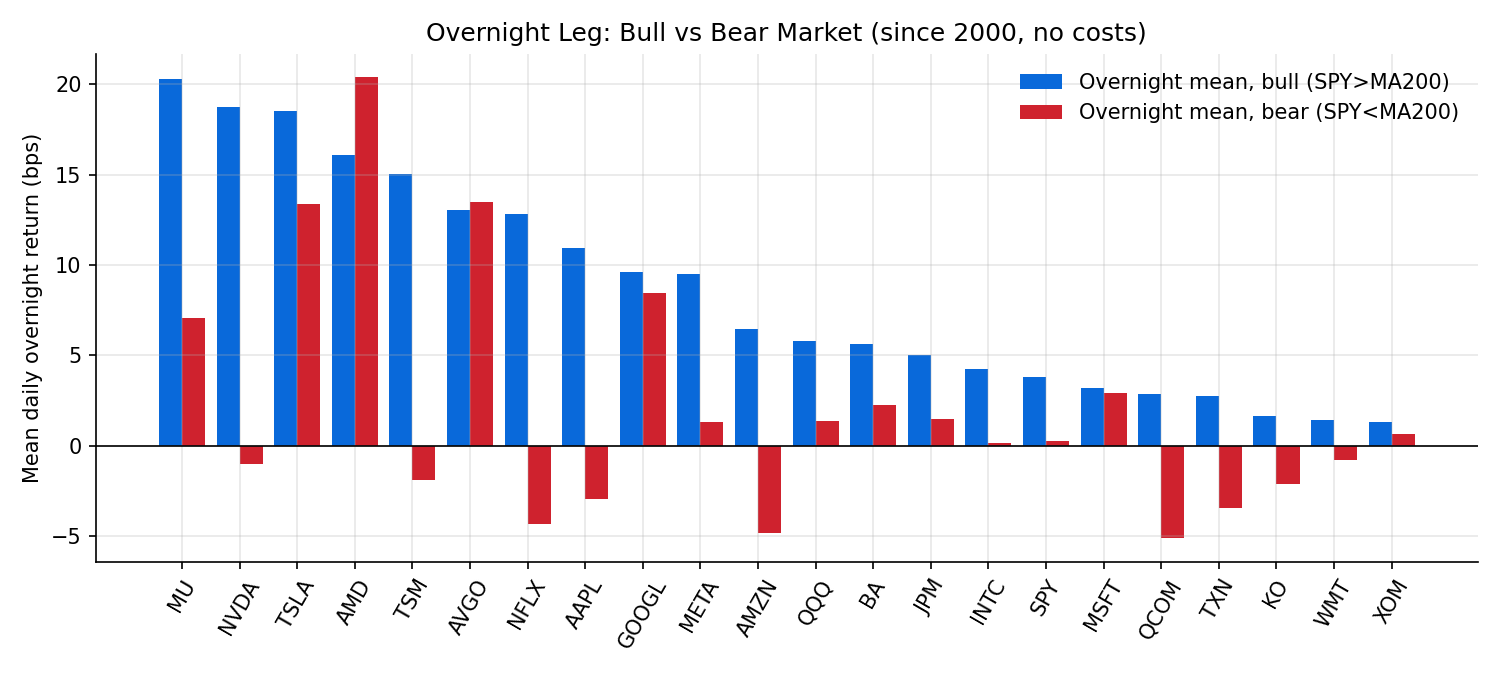
\includegraphics[width=\textwidth]{fig12_bull_bear.png}
\caption{各标的牛市（蓝）vs 熊市（红）夜间日均收益。蓝柱几乎全显著为正，红柱杂乱——熊市夜间收益统计上与零无异。}\end{figure}

\begin{figure}[H]\centering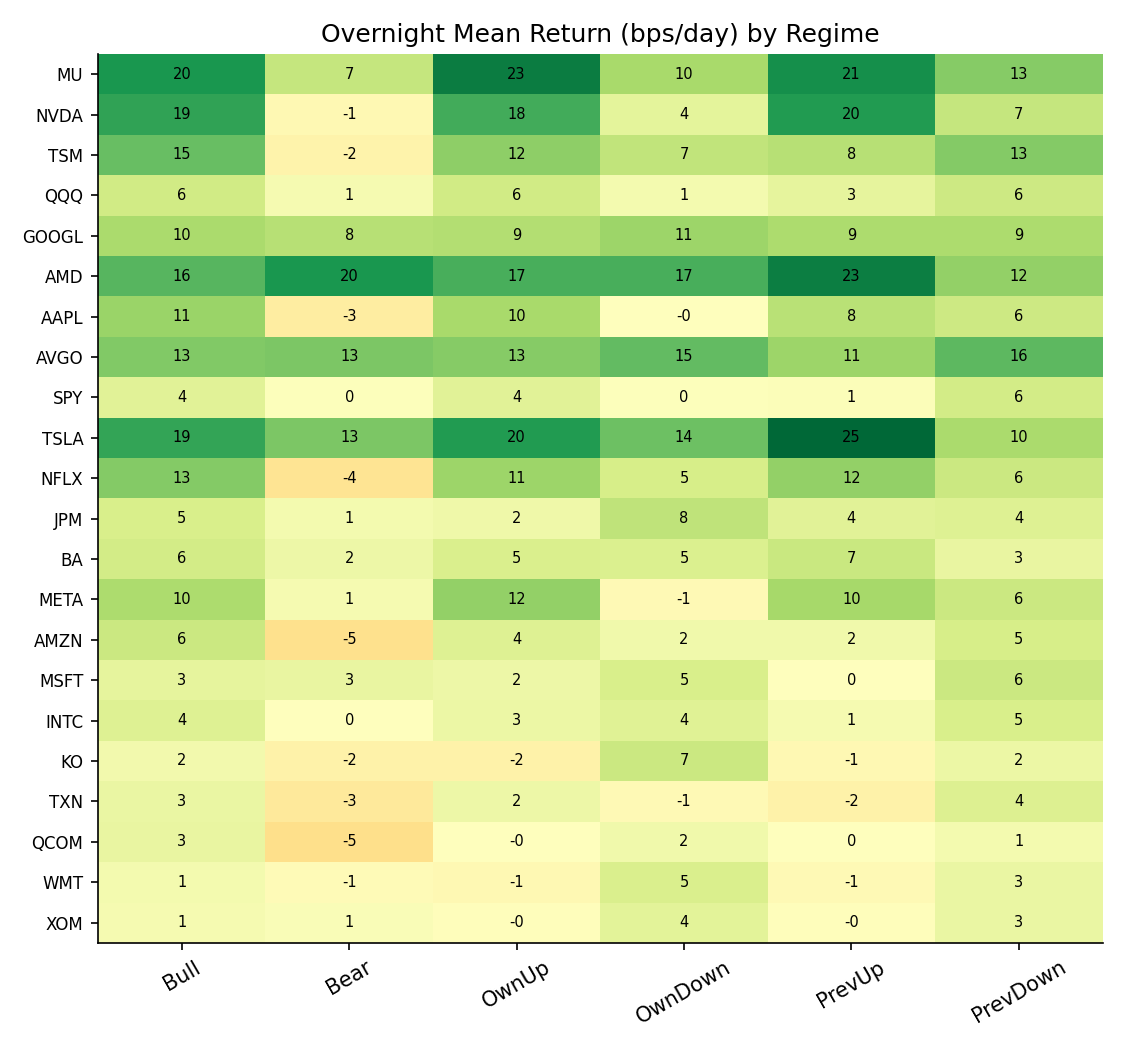
\includegraphics[width=0.75\textwidth]{fig13_regime_heatmap.png}
\caption{状态$\times$标的热力图（夜间日均 bps）。左两列（牛/熊）色差最大。}\end{figure}

\begin{figure}[H]\centering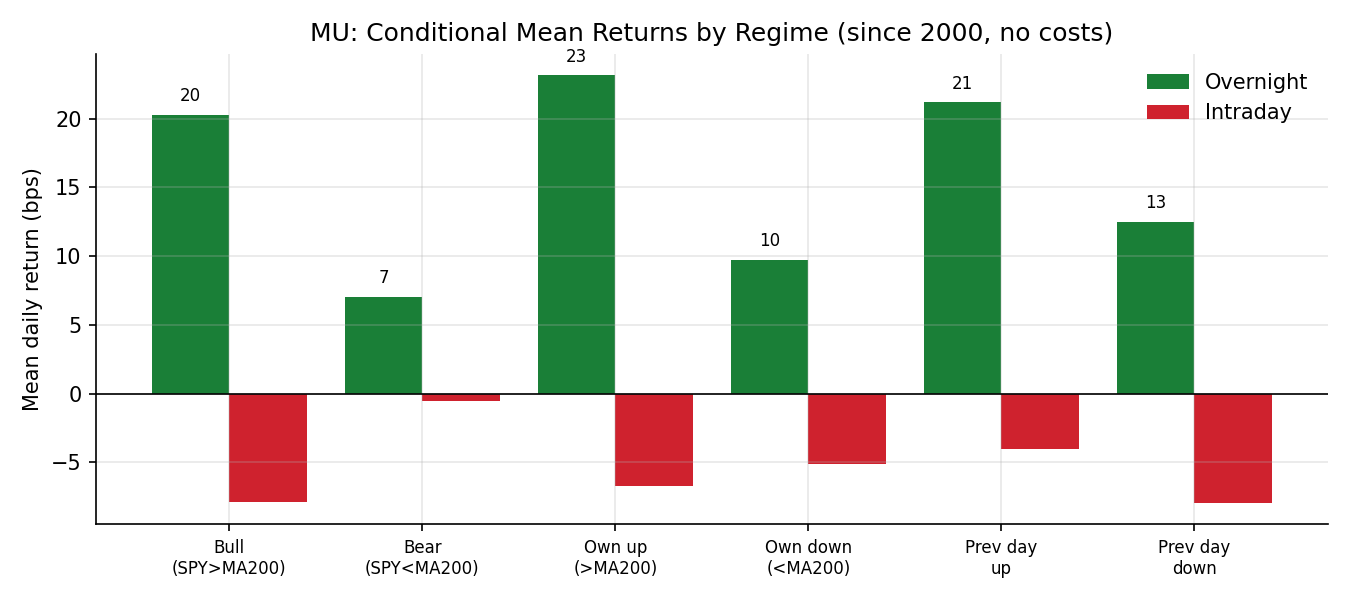
\includegraphics[width=0.92\textwidth]{fig14_mu_conditional.png}
\caption{MU 六状态条件收益。所有状态下夜间为正、日内为负或近零——方向不变，幅度由状态决定。}\end{figure}

%==========================================================
\section{下跌期间：减亏还是扩亏？取决于形态}
\begin{figure}[H]\centering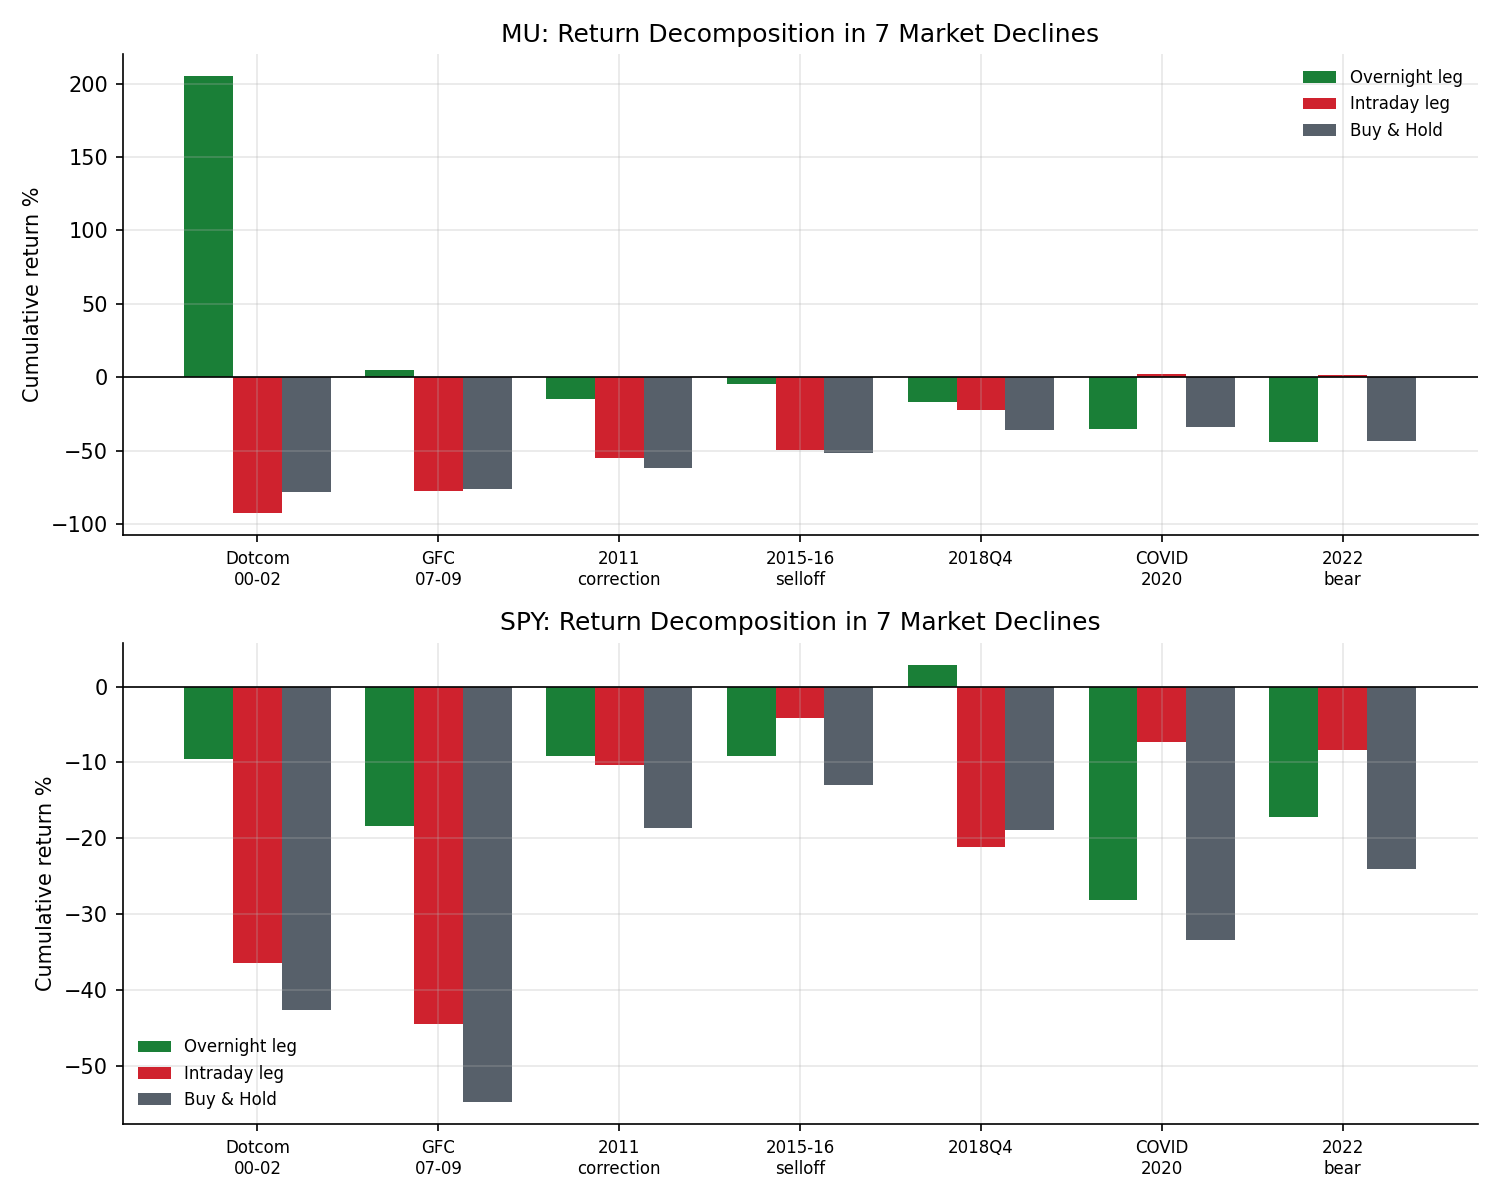
\includegraphics[width=0.92\textwidth]{fig15_crisis.png}
\caption{7 次下跌事件分解（MU 上、SPY 下）。}\end{figure}

\begin{table}[H]\centering\small
\begin{tabular}{lrrl}
\toprule
下跌事件 & 夜间腿 & 买入持有 & 判定 \\
\midrule
互联网泡沫 00-02 & \pos{+205.2\%} & $-$77.9\% & 不止减亏还大赚 \\
金融危机 07-09 & \pos{+5.2\%} & $-$76.0\% & 完全免疫 \\
2011 回调 & $-$14.6\% & $-$61.7\% & 大幅减亏 \\
2015-16 抛售 & $-$4.6\% & $-$51.8\% & 大幅减亏 \\
2018Q4 & $-$17.2\% & $-$35.8\% & 减亏一半 \\
\textbf{COVID 2020} & \negv{$-$35.4\%} & $-$33.8\% & \negv{扩大亏损} \\
\textbf{2022 熊市} & \negv{$-$43.9\%} & $-$43.1\% & \negv{扩大亏损} \\
\bottomrule
\end{tabular}
\caption{\textbf{盘中阴跌型}（前 5 次）夜间持仓是护甲；\textbf{隔夜跳空型}（COVID、2022，坏消息盘后到来）夜间持仓变靶心，且无法止损。MU 单夜最大跳空 $-13.4\%$。}\end{table}

熊市状态几何年化（MU，2000 起）：夜间 \pos{$+10.2\%$} vs 买入持有 \negv{$-12.5\%$} vs 日内 \negv{$-20.7\%$}——平均减亏，但分布两极，无法事先知道下次是哪种形态。

%==========================================================
\section{近端样本外检验：最近 1 个月与 6 个月}
这半年 MU 走出史上最猛单边牛市，是夜间策略\emph{最不利}的环境，正好做压力测试。

\begin{table}[H]\centering\small
\begin{tabular}{lrrr}
\toprule
区间 & 夜间策略 & 日内策略 & 买入持有 \\
\midrule
最近 1 个月 (5/6--6/5) & +29.8\% & +4.0\% & \pos{+35.0\%} \\
最近 6 个月 (25/12--26/6) & +125.5\% & +69.2\% & \pos{+281.5\%} \\
\bottomrule
\end{tabular}
\caption{夜间策略跑输买入持有。\textbf{这不否定论文}：买入持有=夜间$\circ$日内，当日内腿也大正（半年+69\%）时买入持有必然赢，是算术而非反例。}\end{table}

\begin{figure}[H]\centering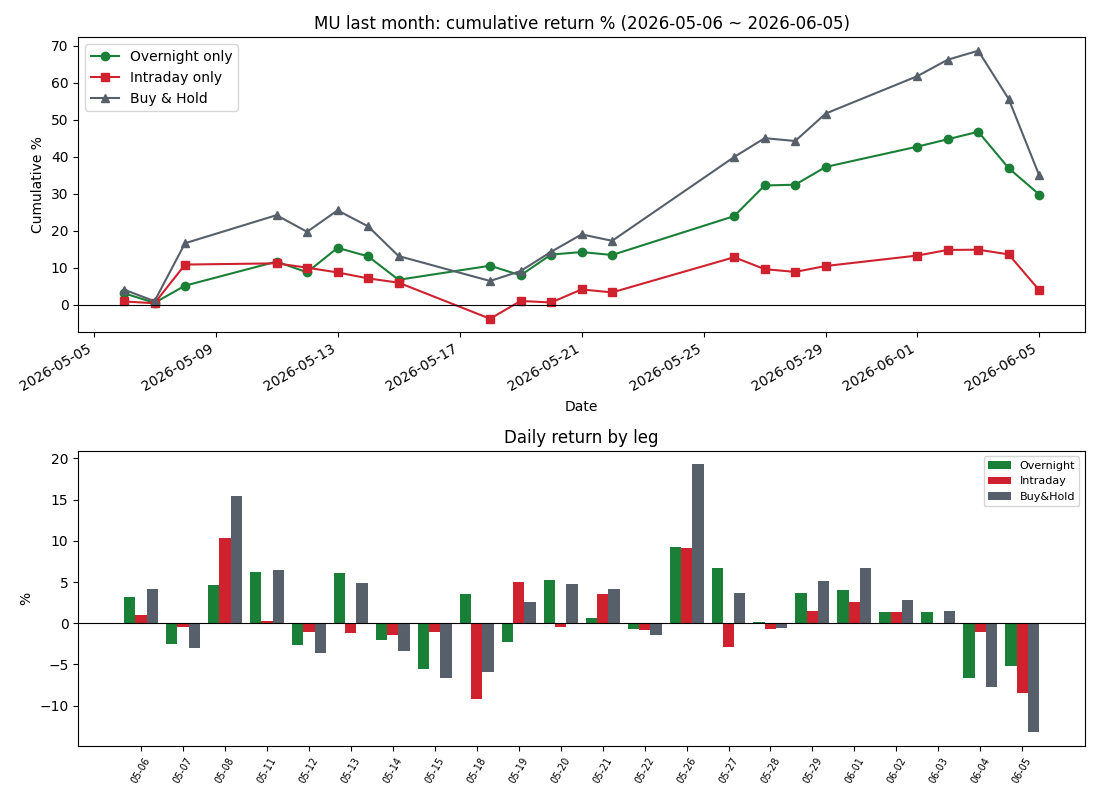
\includegraphics[width=0.93\textwidth]{fig16_recent_month.png}
\caption{最近 1 个月逐日。上涨日夜间仅捕获 61\% 涨幅（5/8 错过 10.9pp、5/26 错过 10.0pp）；下跌日普遍减亏（6/5 少亏 8.1pp）。}\end{figure}

\begin{figure}[H]\centering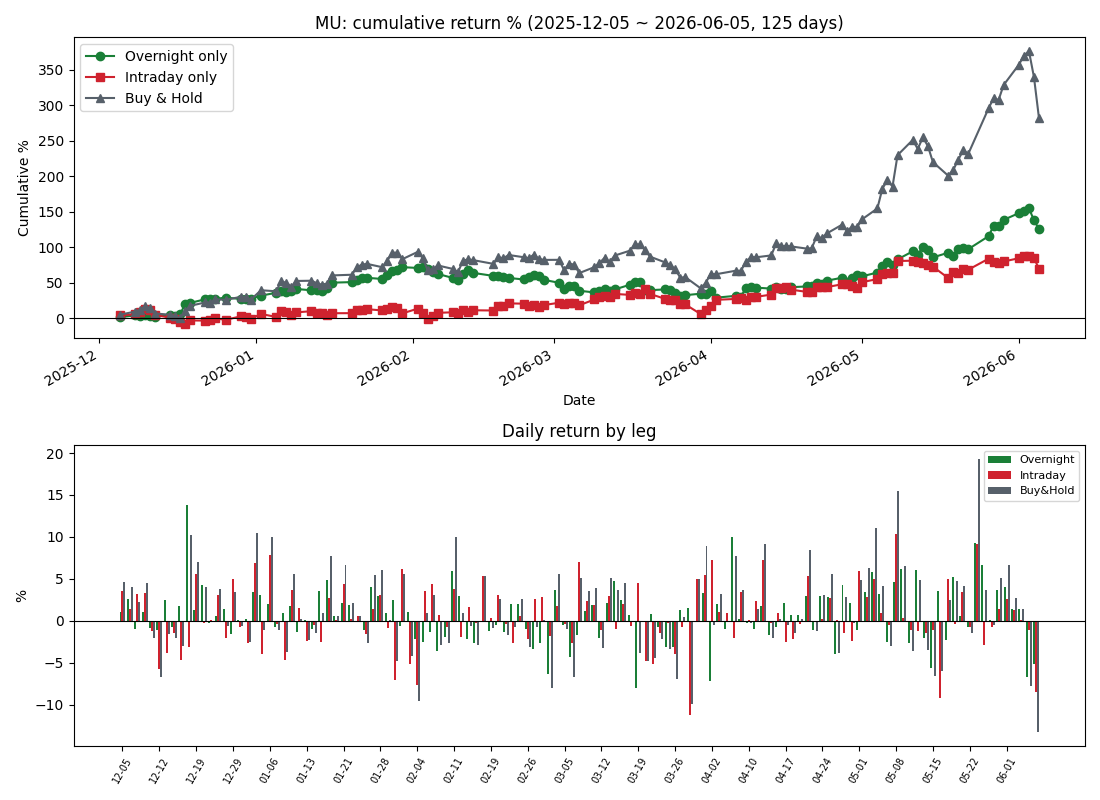
\includegraphics[width=0.93\textwidth]{fig17_recent_6mo.png}
\caption{最近 6 个月。上涨日夜间仅捕获 48\% 涨幅，23 个大跌日中 21 个少亏——\textbf{削峰填谷}：盘中大跌躲过、盘中大涨也踏空。本期盘中净涨，故踏空代价超过减亏好处。}\end{figure}

%==========================================================
\section{策略评估：所有变体横向对比}
\begin{table}[H]\centering\small
\begin{tabular}{lrrrrrr}
\toprule
策略变体（MU 全样本） & Sharpe & Sortino & CAGR & MaxDD & 年化波动 & 累计 \\
\midrule
夜间 0 bps & 1.41 & 1.78 & 42.4\% & $-$54\% & 28\% & 280万$\times$ \\
夜间 2 bps & 1.05 & 1.39 & 28.8\% & $-$69\% & 28\% & 4.07万$\times$ \\
夜间 5 bps & 0.50 & 0.67 & 10.7\% & $-$89\% & 28\% & 71$\times$ \\
\rowcolor{hl} 趋势过滤夜间 0 bps & \pos{1.51} & 1.48 & 30.2\% & \pos{$-$30\%} & 19\% & 6.5万$\times$ \\
\rowcolor{hl} 趋势过滤夜间 2 bps & \pos{1.22} & 1.24 & 23.3\% & \pos{$-$34\%} & 19\% & 6572$\times$ \\
\rowcolor{hl} 趋势过滤夜间 5 bps & 0.78 & 0.80 & 13.6\% & $-$59\% & 18\% & 212$\times$ \\
价差(多夜空日) 0 bps & 0.76 & 1.04 & 31.7\% & $-$99\% & 59\% & 10.4万$\times$ \\
价差(多夜空日) 2 bps & 0.42 & 0.58 & 7.6\% & $-$100\% & 59\% & 22$\times$ \\
价差(多夜空日) 5 bps & \negv{$-$0.09} & $-$0.12 & \negv{$-$20.5\%} & $-$100\% & 59\% & 归零 \\
买入持有 & 0.56 & 0.84 & 16.6\% & $-$98\% & 61\% & 640$\times$ \\
日内 0 bps & $-$0.11 & $-$0.17 & $-$18.1\% & $-$100\% & 53\% & 归零 \\
\bottomrule
\end{tabular}
\caption{\textbf{最优风险调整变体是趋势过滤夜间}（高亮行）：相比纯夜间，回撤近乎腰斩（$-69\%\to-34\%$）、波动从 28\% 降到 19\%、Sharpe 从 1.05 升到 1.22（含 2 bps）。代价是约 47\% 时间空仓，胜率看似下降是因为空仓日不计入。}\end{table}

\begin{figure}[H]\centering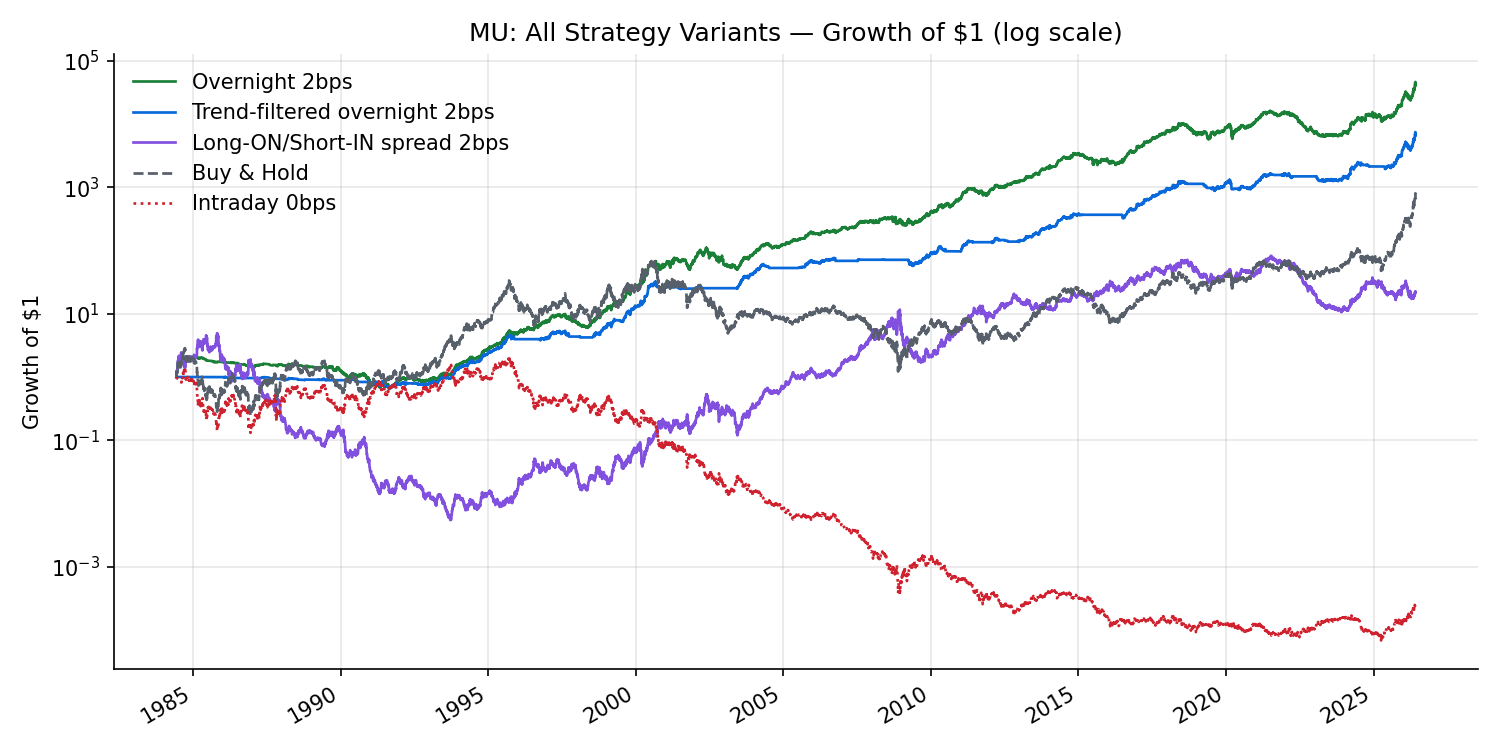
\includegraphics[width=\textwidth]{figA_all_strategies.png}
\caption{全策略变体净值（2 bps，对数轴）。趋势过滤夜间在控制回撤的同时保留绝大部分收益。}\end{figure}

\begin{figure}[H]\centering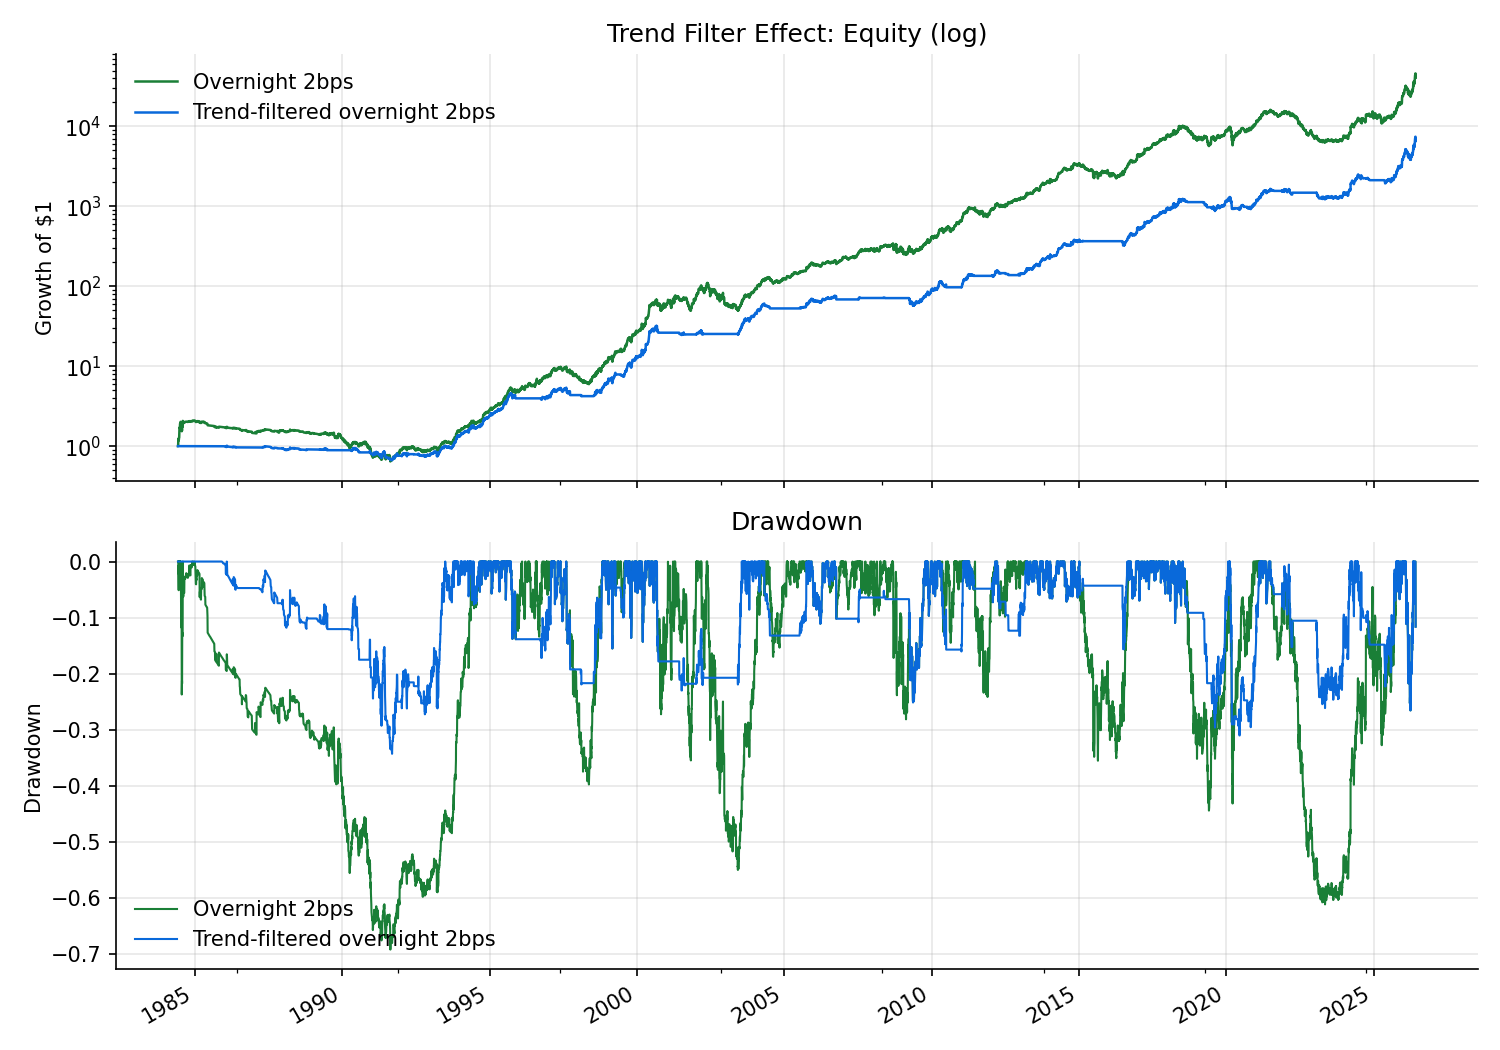
\includegraphics[width=0.92\textwidth]{figB_trend_filter.png}
\caption{趋势过滤效果。上：净值几乎不输纯夜间；下：回撤显著更浅——过滤掉的正是熊市/下降趋势中的隔夜跳空风险。}\end{figure}

\begin{figure}[H]\centering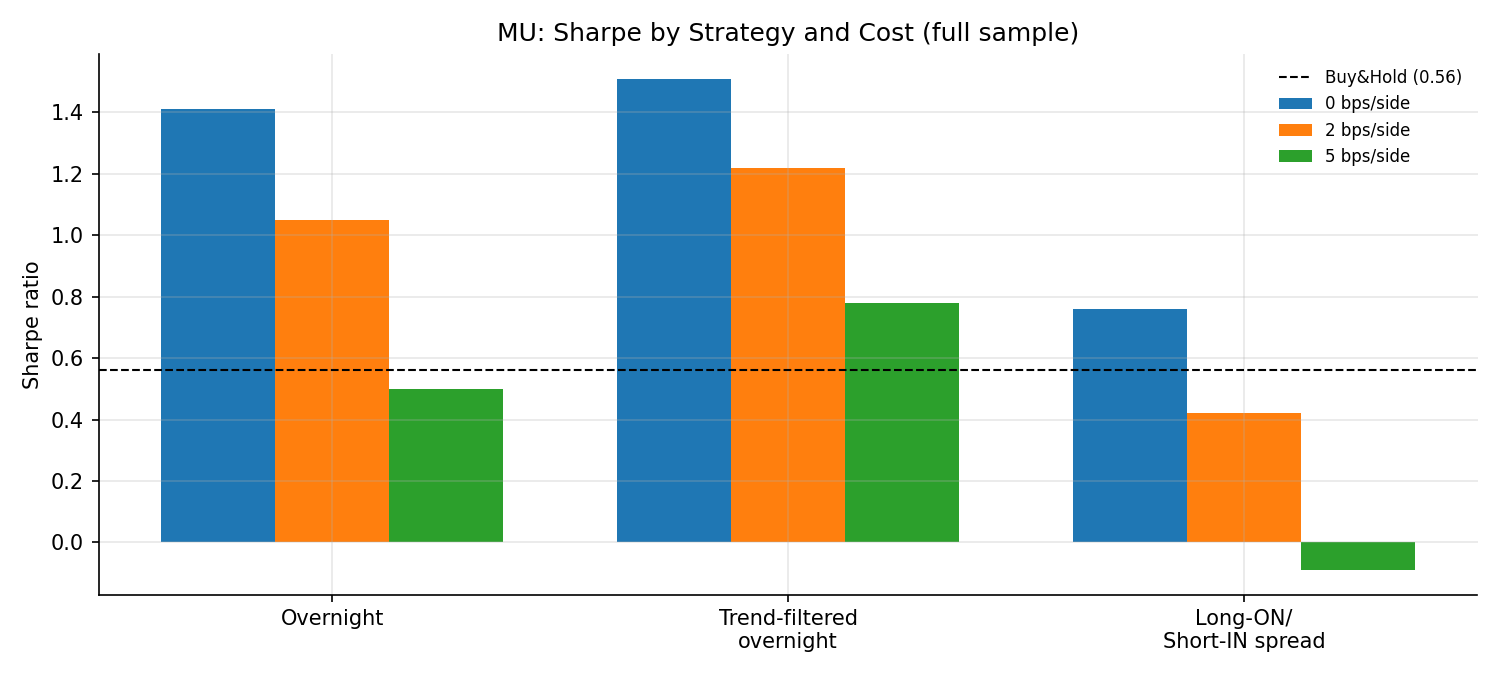
\includegraphics[width=\textwidth]{figD_sharpe.png}
\caption{各策略 Sharpe vs 成本。趋势过滤在每个成本档都优于纯夜间；价差策略全面垫底且 5 bps 转负。}\end{figure}

\begin{figure}[H]\centering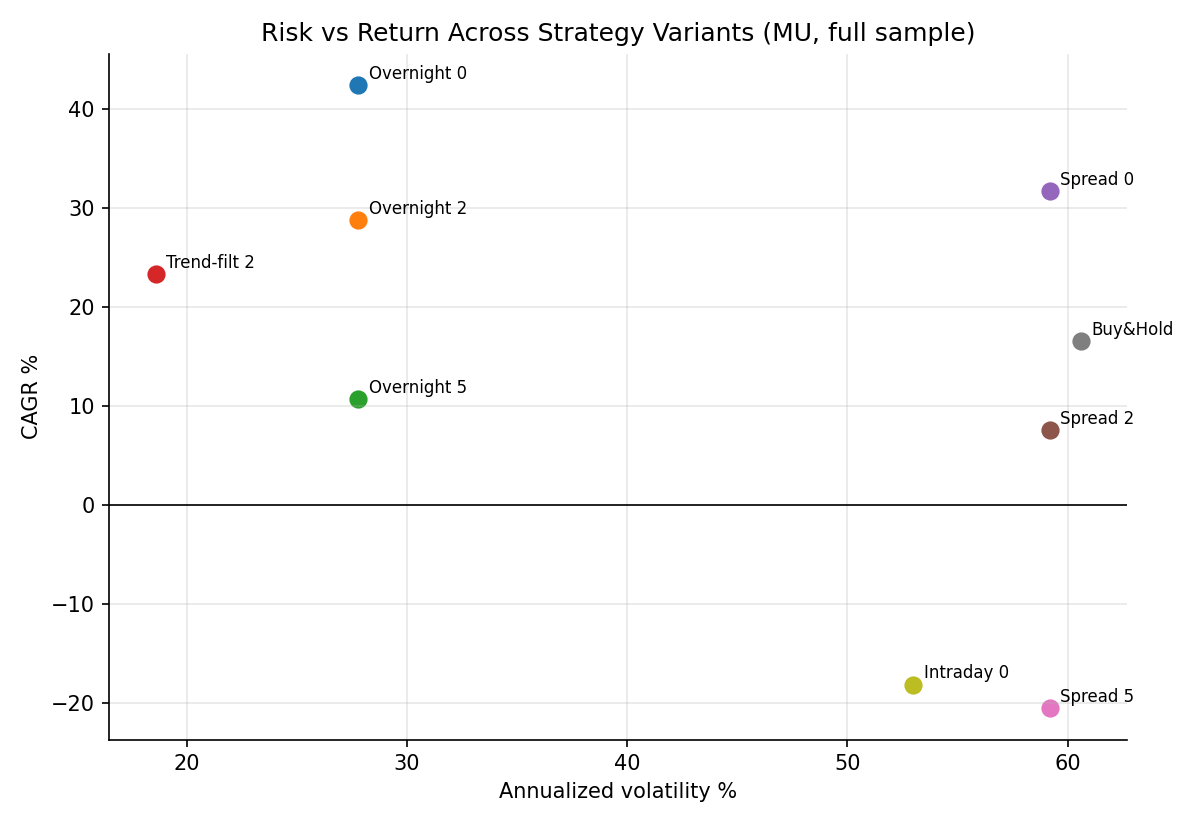
\includegraphics[width=0.82\textwidth]{figE_risk_return.png}
\caption{风险-收益散点。趋势过滤夜间位于左上（低波动高收益）；价差策略偏右（高波动）；日内、价差 5 bps 落入负收益区。}\end{figure}

%==========================================================
\section{"多夜空日"对冲构想的评估：不可行}
\subsection{它是什么}
做多夜盘 + 做空日盘，每日损益 $= r_{\text{on}} - r_{\text{in}}$，是\textbf{市场中性}的价差策略（方向敞口抵消）。\textbf{关键：它不对冲你的方向性 MU 多头}——想保护持仓应用 protective put / collar。

\subsection{为什么散户做不出来}
\begin{figure}[H]\centering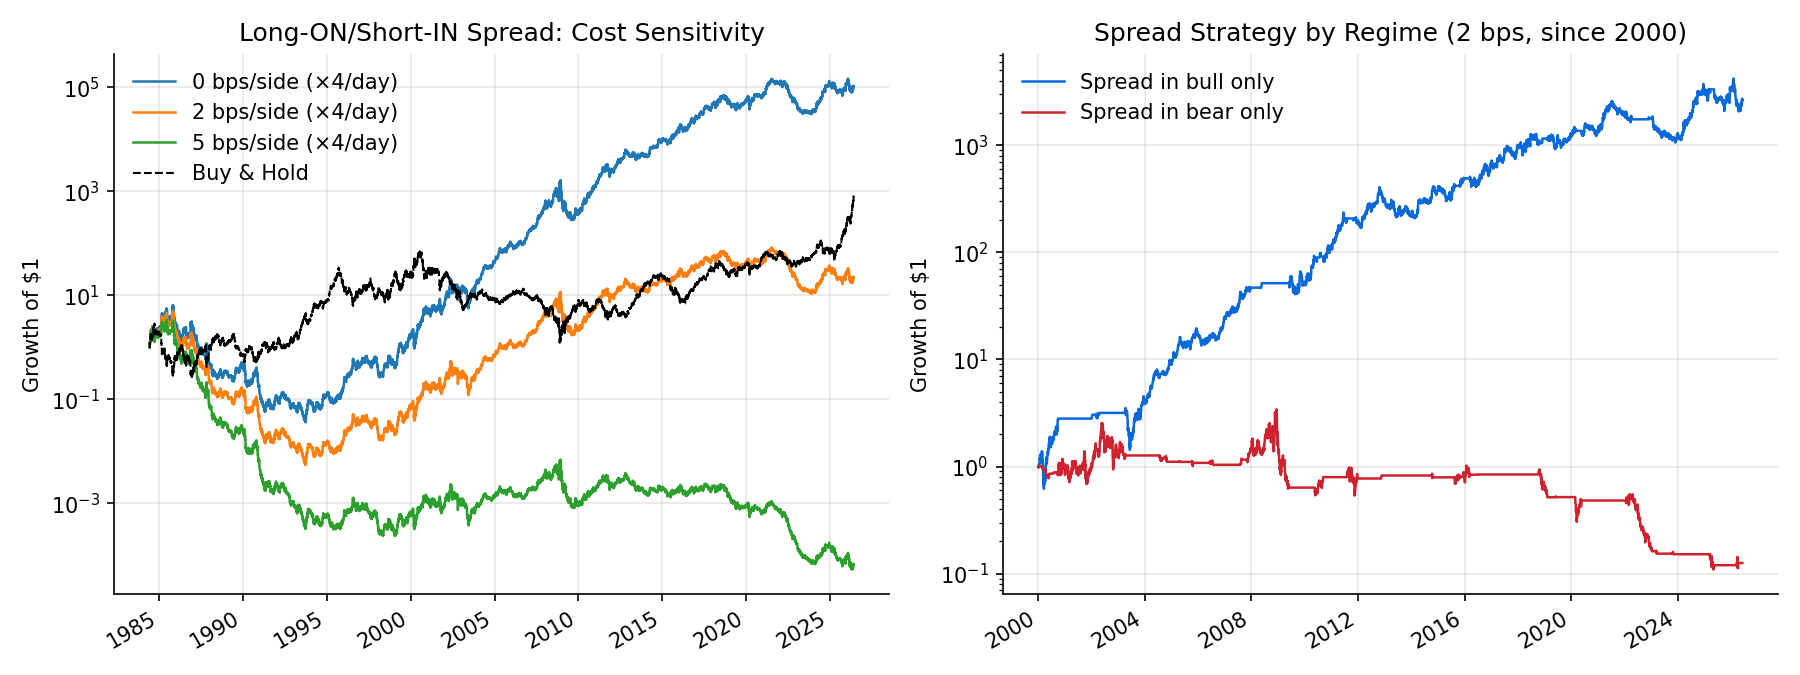
\includegraphics[width=\textwidth]{figC_spread.png}
\caption{左：价差成本敏感性，5 bps 即转负；右：牛熊拆分——牛市 $+20.2$ bps($t=4.92$)，\textbf{熊市 $-0.4$ bps($t=-0.04$) 完全归零}。}\end{figure}

\begin{enumerate}\itemsep2pt
  \item \textbf{换手翻倍}：每天 4 笔成交，盈亏平衡降到 4.5 bps/单边，比单腿（7.8）更难做平；
  \item \textbf{做空一个不显著的腿}：日内腿 $t=-0.73$，统计上等于零——你付双倍成本做空噪声；
  \item \textbf{熊市两腿齐爆}：熊市日内反转为正，做空它反而亏，价差 $t=-0.04$，所谓"对冲"在最需要时塌掉；
  \item \textbf{做空摩擦}：每日 locate、HTB 借不到、uptick 限制、保证金；
  \item \textbf{数据证据}：价差 0 bps Sharpe 仅 0.76（低于纯夜间 1.41），5 bps 转负——\textbf{比单腿更差，不是更好}。
\end{enumerate}

%==========================================================
\section{实操框架}
\subsection{牛熊打法（对持仓者与策略者）}
\begin{table}[H]\centering\small
\begin{tabular}{p{3.4cm}p{4.6cm}p{3.4cm}p{2.8cm}}
\toprule
市场状态 & 持仓者该做 & 执行时点 & 风险动作 \\
\midrule
牛市 + 个股$>$MA200 & 持有，别折腾（买入持有吃两段） & 加仓挂收盘、减仓挂开盘 & 享受隔夜顺风 \\
牛市转弱（跌破个股 MA200） & 开始降杠杆 & 减仓挂开盘 & 优先处理近月期权 \\
熊市 SPY$<$MA200 & 降仓位 / 上对冲（collar、put） & 抄底挂开盘、卖挂收盘 & \negv{绝不裸持隔夜赌跳空} \\
\bottomrule
\end{tabular}
\caption{夜间漂移使开盘价倾向高于昨收，故减仓挂开盘、加仓挂收盘——这是零增量成本、散户唯一够得着的应用。}\end{table}

\subsection{最有价值的不是赚法，是减仓信号}
\textbf{当个股跌破自身 200 日线、且 SPY 也在 200 日线下方 $\Rightarrow$ 夜间"免费顺风"消失 + 跳空风险最高 $\Rightarrow$ 降杠杆/上对冲的客观信号。} 数据背书：该过滤把 MU 最大回撤从 $-69\%$ 砍到 $-34\%$，并自动避开 2022 年 $-49\%$。对策略是放弃收益，对持仓者就是"该减仓的时候"。

\subsection{对集中杠杆持仓者的提醒}
研究能优化\textbf{怎么进出}，救不了\textbf{方向看错}。在刚翻三倍的高波动半导体股上同时押满正股和期权，真正的风险是一次隔夜跳空打穿杠杆。第一问题不是"夜间策略怎么用"，而是"\textbf{若明天 $-50\%$，我能否活下来}"——仓位大小永远比时点重要。

%==========================================================
\section{结论与下一步}
\subsection{核心结论}
\begin{enumerate}\itemsep2pt
  \item 论文（夜间成分长期期望为正）正确，本报告反复证实；网红"1.38 亿\%"误读错误。
  \item 现象在 MU 与多数高波动成长股成立，但盈亏平衡 7.8 bps/单边，零售直接套利大概率无利可图。
  \item 本质是牛市现象；熊市对下跌的保护取决于"盘中阴跌"还是"隔夜跳空"，后者无效且无法止损。
  \item 最实用产出是\textbf{趋势过滤}（风险大幅下降）与\textbf{执行时点优化}（零成本边际改进）。
  \item "多夜空日"价差是中性策略而非方向对冲，散户经济性不成立。
\end{enumerate}

\subsection{升级到可交易级仍需}
分钟级数据测真实滑点（开/收盘前后 5 分钟 VWAP）；MOO/MOC 竞价单事件驱动模拟（LEAN）；税务（短期资本利得）与融资/借券成本；组合化（等权一篮子高波动半导体股替代单票）；样本外验证（2020 前定参、后验证，重点查 2022 式反转）。

\appendix
\section{局限性声明}
\begin{itemize}\itemsep0pt
  \item 开/收盘成交为理想化假设，真实可成交价更差；Yahoo 早年开盘价质量存疑（部分为复制值）；
  \item 单票分析有选择偏差（MU 因效应极端被论文选中）；横截面为手选 22 票，非全市场；
  \item 价差策略成本按每日 4 笔近似（$r_{on}-r_{in}-4c$），未计借券费与 locate 失败；
  \item 趋势过滤胜率下降系空仓日不计入所致，非择时变差；MA200 为滞后指标，状态切换初期仍吃最剧烈跳空；
  \item 2026 年为不完整年度；未考虑停牌、退市、流动性枯竭。
\end{itemize}

\vspace{0.8em}
\noindent\small 代码与数据：\texttt{research/overnight/}（\texttt{backtest\_overnight.py}、\texttt{make\_report\_assets.py}、\texttt{regime\_analysis.py}、\texttt{crisis\_analysis.py}、\texttt{recent\_month.py}、\texttt{final\_assets.py}）。
参考：Lou, Polk, Skouras (2019), \textit{A Tug of War: Overnight versus Intraday Expected Returns}, Journal of Financial Economics.
\end{document}
